\documentclass[a4paper]{article}
\usepackage[T1]{fontenc}
\usepackage[utf8]{inputenc}
\usepackage[italian]{babel}
\usepackage{amssymb}
\usepackage{hyperref}
\usepackage{mathtools}
\usepackage{amsthm}
\usepackage[ruled,vlined,noend]{algorithm2e}

\mathtoolsset{showonlyrefs}  
\hypersetup{
    colorlinks=true,
    linkcolor=black,
    filecolor=black,      
    urlcolor=black,
}
\newcommand{\argmin}{\operatornamewithlimits{argmin}}
\newcommand{\pluseq}{\mathrel{{+}{=}}}

\newtheorem{theorem}{Teorema}
\newtheorem{corollary}{Corollario}
\newtheorem{lemma}{Lemma}
\newtheorem{remark}{Osservazione}
\newtheorem{definition}{Definizione}

\setcounter{secnumdepth}{3}
\setcounter{tocdepth}{3}

\title{Algoritmica per il web}
\author{Francesco Tomaselli}
\makeindex
\begin{document}
\maketitle
\newpage
\tableofcontents
\setlength{\parindent}{0pt}
\setlength{\parskip}{0.8em}
\newpage
\section{Crawling}

\subsection{Principi di base}

\paragraph{Insiemi di nodi in una visita}
All'interno di un processo di crawling, si distinguono 
tre insiemi di nodi 
\begin{itemize}
    \item $U$: nodi sconosciuti 
    \item $F$: frontiera, ovvero nodi che sono conosciuti ma non ancora visitati
    \item $V$: nodi visitati
\end{itemize}
Una visita del web opera scegliendo un nodo della frontiera, 
aggiungendolo ai visitati, e aggiungendo i siti raggiungibili da esso alla frontiera.

In una visita di un grafo classica, gli insiemi $U$ e $F$ coincidono nel secondo.
\begin{remark}
    Teoricamente una visita potrebbe esaurire la frontiera, 
    praticamente non finisce mai, a parte in rari casi.
\end{remark}

\paragraph{Inizializzazione frontiera}
La frontiera va inizializzata, tipicamente si scelgono siti web popolari, 
per esempio giornali etc. In generale si considerano \emph{semi} di inizializzazione, 
ovvero un insieme di siti web scelti da umani, che sono promettenti.

La scelta del seme governa l'esplorazione della frontiera, 
verranno scelti infatti prima siti più vicini ai siti di inizializzazione.

Un'altra strada per la frontiera è scegliere a priori un insieme di siti 
web, e considerarla direttamente come frontiera, tralasciando i siti 
raggiungibili da essi. 

\subsection{Strutture dati}

\paragraph{Strutture in memoria}
Sono cruciali le strutture usate per memorizzare i nodi visitati 
e la frontiera.

Mantenere i visitati in una hashtable è ragionevole, non lo è 
per la frontiera, tipicamente di ordini di grandezza più grande dell'insieme $V$.

Limitare la grandezza della frontiera è cruciale, si potrebbere preferire 
i link iniziali in una pagina piuttosto che quelli a fondo. Oppure limitare 
il numero massimo di pagine estratte da un singolo dominio o considerare 
un limite alla profondità all'interno di un singolo sito web.

\paragraph{Scelta del prossimo nodo}
Ciò che determina il comportamento una visita di crawling è 
la scelta del prossimo nodo della frontiera. Una scelta ragionevole 
potrebbe essere una visita in ampiezza a partire dalla frontiera iniziale.
L'assunzione è che pagine di qualità puntino ad altre pagine di qualità.

Operare in profondità non funziona, significherebbe continuare a scendere 
all'infinito, al contrario di una classica DFS che termina e si \emph{torna indietro} 
con la ricorsione. Questo perchè i siti non visitati sono praticamente infiniti.

Criteri più sofisticati possono associare una sorta di priorità alle pagine. 
Tali criteri sono legati ai contenuti delle pagine, alla struttura dell'url, 
alcuni esempi sono:
\begin{itemize}
    \item Url corti, con l'assunzione che i livelli siano separati da un backslash;
    \item Url fuori dal sito corrente;
    \item Parole chiave di interesse all'interno dell'url;
    \item Utilizzo il contenuto della pagina corrente per avere informazioni 
    sulla pagina successiva.
\end{itemize}
In questo caso si utilizza una coda a priorità, con qualche valore di priorità 
associato ad ogni nodo.

\begin{remark}
    In questo paragrafo si sta assumendo un contesto single thread, ovviamente nella realtà si 
    utilizzerà un approccio multithread, e molti fattori, quali latenza, 
    tempi di risposta, race condition, influenzano sull'ordine di visita effettivo.
\end{remark}

\subsubsection{Esempio strutture dati}

\paragraph{Visti hashati}
Una prima idea per mantenere l'insieme $V$ è non memorizzare url completi ma una certa firma digitale 
di essi. 

Consideriamo ad esempio una funzione di hash:
$$f : \mathit{URL} \longrightarrow 2^{64} = \{0, \dots, 2^{64-1}\}$$
È possibile che due url collidano, creando errori sui positivi, ovvero un 
url non davvero visitato viene visto come già esplorato.

Solitamente le collisioni non importano, ma, dati $k$ elementi contenuti 
nella struttura, data una funzione di hash buona, tipicamente il numero di collisioni 
è dell'ordine di $\frac{k^2}{2n}$, dove $n$ è la grandezza del codominio. 

Nella pratica quindi, funzioni di hash come $f$, non creano un numero 
spiacevole di collisioni.
\begin{remark}
    Una tabella di firme è molto più efficiente di mantenere i dati effettivi, 
    basti pensare a problemi di allocazione di memoria inefficiente, frammentazione 
    etc.
    Pagare il prezzo dei conflitti, implica risparmiare molti problemi e spazio.\\
    Mantenere una tabella di firme significa di fatto mantenere in memoria strutture 
    più piccole dell'information theoretical lower bound, pagando il prezzo delle collisioni.
\end{remark}

\paragraph{Database NoSQL}
Sono  database che memorizzano entry chiave valore, 
un esempio è \emph{RocksDB}. Se ordinati sono implementazioni efficienti di B-Tree, 
altrimenti di dizionari classici, in parte memorizzati su disco. 

Si utilizzano anche LSM-Tree, alberi che dividono per livelli le chiavi e mantengono 
chiavi utilizzate di frequente all'inizio, spostando chiavi poco frequenti nei 
livelli più bassi.

\subsection{Crivelli}

Un crivello è una struttura dati che accetta le seguenti primitive: 
\begin{itemize}
    \item \emph{add(u)}: aggiunge un url alla struttura;
    \item \emph{get()}: preleva un elemento dalla struttura. 
\end{itemize}
Un crivello ha un aspetto insiemistico, ovvero ricorda cosa è stato inserito 
o no, gestisce anche l'ordine in cui restituisce i dati, tipicamente 
si considera una visita in ampiezza. 

Un' implementazione base è un' hashtable in memoria, per i già visti, ovvero $V \cup F$, 
e una coda in memoria per gestire l'ordine di visita, BFS nel caso di una coda classica.

\begin{remark}
    È necessario comunque del processing degli url estratti dal crivello, ad esempio, 
    potremmo ordinarli per dominio, in modo da raggruppare richieste allo stesso sito.
\end{remark}

\paragraph{Implementazione}
È già stata accennata la possibilità di avere una hashtable più una coda. 
L'hashtable potrebbe, come introdotto a sottosezione precedente, solo le firme degli url, in modo da ridurre lo spazio in memoria necessario.

\paragraph{Graceful degradation}
È importante garantire il \emph{graceful degradation}, ovvero, il sovraccarico della 
struttura ne peggiora le performance ma non fa crollare l'intero processo. 
Una struttura dati classica, come una hashtable, non garantisce questa proprietà, 
al termine della memoria essa fallisce.

\subsubsection{Filtri di Bloom}
Un filtro di Bloom è un dizionario approssimato, che garantisce una certa probabilità di errore positivo assumendo un certo upper bound al numero di chiavi inserite. 

L'impronta in memoria di un filtro di questo tipo è costante, non varia quindi al variare 
del carico della struttura.

\paragraph{Funzionamento}

Sia $b$ un vettore di $m$ bit, sia $d$ il parametro che regola la precisione del filtro,
e $f_i : U \rightarrow m, 0 < i < d$ funzioni di hash che mappano un elemento dell'universo 
in un indice del vettore. 

Le primitive disponibili sono, dato $x \in U$: 
\begin{itemize}
    \item \emph{add(x)}: imposto ad uno le posizioni date dalle funzioni di hash, 
    ovvero $f_0(x), \dots, f_{d-1}(x)$;
    \item \emph{contains(x)}: restituisco l'and logico delle posizioni $b[f_i(x)]$.
\end{itemize}

L'operazione contains restituisce zero se e solo se $x$ non è stato inserito nel filtro. 
Un risultato positivo però può significare che $x$ sia stato inserito oppure che 
inserimenti precedenti abbiano settato ad uno tutte le celle relative agli hash di $x$.

\paragraph{Probabilità di falsi positivi}
Se fissiamo $d$ ad uno non si sta guadagnando rispetto ad una classica tabella di hash.
Più $d$ è grande, più sono improbabili i falsi positivi, ma più uni si vanno ad aggiungere, quindi i falsi positivi aumentano.

Bisogna quindi trovare un tradeoff tra $m$ e $d$ per minimizzare la probabilità di falsi positivi.
Si considera ora un $n$, ovvero il numero di chiavi inserite. 

Si ottiene che la probabilità di un falso positivo equivale a $\frac{1}{2}^d$ e la 
dimensione $m = 1.44 dn$. 
Questo implica che fissata una precisione e il numero di chiavi massimo, si può ottenere lo 
spazio necessario, similmente, fissato $m$ e $n$ si può ottenere la precisione ottenuta.

\begin{remark}
    La struttura ha degrado grazioso, infatti, eccedendo $n$ l'analisi di precisione non vale più e 
    i falsi positivi aumentano. Si nota anche che sotto la soglia $n$ la probabilità di falsi 
    positivi diminuisce. 
    La struttura non fallisce, peggiora in precisione fino a che è satura, restituendo sempre positivo.
\end{remark}
\begin{remark}
    Gli accessi in cache sono pessimi per quanto riguarda un filtro di bloom, 
    dovendo controllare celle di memoria non correlate e sostanzialmente casuali, 
    quindi con poca probabilità di essere in cache.
\end{remark}
\begin{remark}
    I risultati negativi in media accedono a solo due celle.
\end{remark}

\paragraph{Blocked Bloom filter}
Si può pensare di dividere un filtro di Bloom in due filtri più piccoli di dimensione $1.44d\frac{n}{2}$ ciascuno.
Una funzione $g$ sceglie quale filtro scegliere, poi, si inserisce l'elemento nel filtro selezionato.

La divisione permette di mantenere i filtri in cache e velocizzare il tutto. 
Un'analisi avanzata individua un degrado di precisione. Questo perché alcuni filtri 
mantengono poche chiavi, ed altri saranno più sovraccarichi.

\paragraph{Calcolo funzioni di hash}
Supponendo di avere due funzioni di hash $h(x)$ e $g(x)$, siano $a = h(x)$ e 
$b = g(x)$, considerando l'i-esima funzione di hash come $ai + b$, 
l'analisi sulla precisione di falsi positivi rimane valida. 
\begin{remark}
    Il calcolo fatto in questo modo è estremamente più efficiente di calcolare 
    $d$ funzioni separate. 
\end{remark}

\subsubsection{LMS tree}
Un \emph{Log-Structure-Merge} tree memorizza file di log in cui si scrive solo in append. 

A differenza di un classico \emph{B-tree}, i registri non cambiano.
Questi alberi funzionano molto bene quando si scrive molto e legge poco.

\paragraph{Livelli}
L'idea di base di un \emph{LMS} tree è avere un certo numero di livelli nella struttura 
dati. Idealmente i vari livelli possono essere mantenuti in mezzi di memorizzazione 
differenti. 
Si assume ora che il primo livello sia in memoria, in una struttura classica 
come un B-tree e i successivi su disco come registri di coppie chiave-valore ordinate. 

Ogni livello ha memorizzate un certo numero di coppie chiave-valore, ed ogni livello successivo occupa 
dieci volte più del precedente. 

\paragraph{Ricerca}
Per trovare una chiave, si cerca nei livelli in maniera sequenziale, 
una volta individuata, al livello più alto possibile\footnote{Potrebbe comparire 
anche in livelli successivi, visto che si ammettono duplicati}, si restituisce.
Visto che le chiavi sono ordinate, si potrebbe effettuare una ricerca 
dicotomica\footnote{Bisogna stare attenti al tipo di memoria, a volte accessi sequenziali 
sono molto più veloci di accessi aleatori, un esempio è nel nastro.}.

\paragraph{Inserimento}
L'aggiunta all'albero inserisce la chiave al livello zero. Se la chiave non è presente il B-tree sale di dimensione, se eccede la dimensione massima: 
si considera un segmento contiguo di chiavi e si fondono con il livello uno\footnote{La fusione 
è molto veloce essendo le due strutture ordinate}.
Si procede fino a che non si trova un livello che riesce a mantenere le chiavi. 
Se si raggiunge l'ultimo livello, se ne crea uno nuovo. 

Il principio di base è che le fusioni dei livelli, che sono molto costose, avvengono sempre 
più raramente allo scendere nell'albero.

\paragraph{Rimozione}
La rimozione consiste nella ricerca della chiave e nella sostituzione del suo 
valore con una \emph{tombstone}. Una ricerca successiva troverà questo valore e capirà 
che la chiave è stata rimossa.

\paragraph{Frammentazione livelli}
Ogni livello nella pratica è frammentato in tanti file piccoli. Questo offre 
molti vantaggi, ad esempio operazioni di merge parallele. Inoltre, favorisce 
l'evitare collisioni di concorrenza. 

La ricerca poi è più veloce, poiché è 
possibile mantenere un indice sparso, con un sottoinsieme di chiavi, con puntatori 
ai frammenti relativi alla chiave. Ogni livello ha poi un filtro di Bloom.
La ricerca quindi testa il filtro e se la risposta è negativa si procede al 
livello successivo, altrimenti, si controlla l'indice sparso in ricerca dicotomica, 
e si procede sequenzialmente dalla maggior chiave minore uguale di quella ricercata.

\subsubsection{Crivello offline} 
Si mantengono solo file su disco e non strutture in memoria. 
I file vengono ordinati e fusi spesso. In particolare, si hanno a disposizione: 
\begin{itemize}
    \item \emph{Z}: url già visti, $V \cup F$
    \item \emph{F}: frontiera, ovvero gli url da visitare
    \item \emph{A}: file che accumula gli url incontrati durante la visita
\end{itemize}

All'inizio $Z$ ed $F$ sono inizializzati con il seme ed $A$ è vuoto.
Durante la visita si estrae con qualche criterio da $F$, accumulando in $A$, 
quando si esaurisce il primo o il secondo è pieno:
\begin{enumerate}
    \item $A$ viene ordinato e deduplicato, diventa $A^\prime$;
    \item $Z$ diventa $Z^\prime$ pari all'unione di  $A^\prime$ e $Z$: 
    durante la fusione gli url che compaiono in $A^\prime$ ma non in $Z$ vengono 
    aggiunti ad $F$.
\end{enumerate}

Il punto due ha complessità lineare, visto che i due file sono ordinati, 
l'ordinamento di $A^\prime$ disordina gli url per quanto riguarda l'ordine di accodamento, 
per ovviare al problema si potrebbe mantenere nel file oltre che l'url, la posizione originale
di accodamento, in modo da riordinarli una volta accodati ad $F$.

$Z$ potrebbe contenere firme al posto di url, in questo caso $A$, che contiene url, 
va ordinato indirettamente per firma.

Al crescere della frontiera il crivello diventa lento ma non si blocca, ha perciò graceful 
degradation.

\paragraph{LRU cache}
Può essere una buona idea anteporre al crivello una cache LRU, questo rimuove 
molti duplicati, infatti se un url è all'interno della cache è già stato inserito 
all'interno del crivello. \\
Ogni tanto un url verrà inserito più volte, perché finito fuori dalla cache.

\subsection{Quasi duplicati}
Per molteplici ragioni, è possibile incontrare spesso le stesse pagine, 
per esempio, la stessa pagina con http e https, pagine che differiscono per una 
sola data, etc.\\
È necessario un sistema che decida se due pagine sono quasi identiche.

\paragraph{Digest}
Si puo generare un digest dalla pagina web, buttando via alcuni elementi, 
per esempio i tag html, le maiuscole, etc.
Si può anche campionare la pagina in qualche intervallo e memorizzare solo 
i campionamenti.
Una volta generati questi digest saranno inseriti in un filtro di Bloom.

\paragraph{SimHash}
L'idea di base è generare hash simili per testi simili. La distanza tra due testi 
si misura in distanza di Hamming.
Si risolvono problemi come ad esempio il considerare due pagine diverse per un 
singolo errore ortografico.

A partire dal testo si ottengono delle feature da esso. Un esempio potrebbe essere 
estrarre le parole, oppure considerare tre-gram da esso, ovvero sotto-sequenze di tre 
caratteri o magari tre parole alla volta, etc.
N-gram corti implicano il non considerare troppo importanti errori di ortografia.

Siano ora $s \in S$ le feature estratte e $h : \mathit{Stringhe} \rightarrow 2^b$ funzione 
di hash.
Consideriamo ora il valore di hash per ogni feature, $h(s)$, l'hash finale del documento 
si ottiene contando la maggioranza per ogni bit degli hash delle feature, per esempio: 
\begin{itemize}
    \item $s_0$ : $1,0,1,1,0$;
    \item $s_1$ : $0,1,0,0,1$;
    \item $s_2$ : $0,1,0,1,1$;
\end{itemize}
L'hash finale del documento sarà: $0, 1, 0, 1, 1$

Il calcolo effettuato in questo modo sistema i casi di poche differenze tra i testi, 
dipende ovviamente dalle feature che si considerano, ma è auspicabile che poche 
feature differenti tra due documenti non modifichino i voti di maggioranza, oppure, che influiscano su pochi bit. 

\subsection{Politeness}

Dal punto di vista etico, una persona che mette una pagina sul web 
deve accettare che sarà visitata, da umani. 
La visita e l'indicizzazione automatica tramite crawler non dovrebbe 
continuare per periodi troppo prolungati.

\paragraph{Politeness assoluta}
Intervallare di un certo numero di secondi le richieste consecutive ad 
un sito, oppure allo stesso ip. Esempio, faccio 10 richieste, pausa di qualche secondo, altre 10 richieste.

\paragraph{Politeness relativa}
Per un certo intervallo di tempo scarico tutto quello che posso. Poi mi 
adatto in base a come la pagina ha risposto, ad esempio, 
scarico per un secondo tutto quello che riesco, ma la pagina impiega 
10 secondi a rispondere, aspetto quindi 30 secondi prima di effettuare 
una nuova richiesta.

Potrei usare HTTP 1.1, per mantenere aperta la connessione. 

\begin{remark}
    È necessaria un'architettura multiflusso per raccogliere dati 
    da molti siti contemporaneamente, altrimenti si aspetterebbe molto 
    per ragioni di politeness e si diventerebbe troppo dipendenti 
    dall'ordine della coda dei siti da visitare, infatti, dovrei aspettare 
    se il prossimo sito fosse nello stesso dominio di quello attuale, no altrimenti.
\end{remark}

\paragraph{Robots.txt}
File che deve comparire nella radice di un sito web dove si possono 
escludere parti di sito da visitare.
Se uno ignorasse i contenuti del file probabilmente sarebbe bannato. 

\subsection{Concorrenza}
Ogni host estratto dal crivello ha una coda con gli url relativi ad esso. 
Bisogna quindi ora capire quale host considerare e visitarne gli url associati.

Visite ad host diversi possono essere fatte in concorrenza, per capire 
quale host è disponibile, secondo le regole di politeness, si utilizza una priority queue.

\subsubsection{Componenti di un crawler}

\paragraph{Coda di host}
Si considera una coda di host, ordinati per tempo da aspettare 
prima di poter scaricare dal sito. 

Se il sito in testa ha tempo minore uguale a quello attuale esso si estrae, 
si scaricano tutti i siti che si riescono da quell'host, poi si reinserisce 
in coda con timestamp uguale al tempo attuale più intervallo di politeness.

La coda è gestita da un semaforo per permettere concorrenza.

\begin{remark}
    Considerando una dimensione massima per la coda potrei dover
    escludere dei siti se il timer crescesse troppo. Sta a chi progetta 
    il crawler decidere se potare la coda nel caso in cui cresca troppo in 
    memoria.
\end{remark}

\paragraph{Coda di ip}
Il discorso si complica nel caso si considerino gli ip. 
Si considera una coda di ip con un timestamp,\footnote{Si può assumere
un timer di politeness di 10 secondi.}, ogni ip ha una coda di host 
come quella presentata in precedenza.
Il timestamp dell'ip equivale al massimo tra il timestamp suo e quello 
della testa della sua coda di host.

Una volta individuato l'ip da estrarre si estrae dalla coda e si procede 
come in precedenza.
Questo garantisce di rispettare la politeness anche verso ip con molti 
host associati.

\paragraph{Fetching e parsing threads}
Nella pratica ci sono fetching thread che scaricano secondo le policy descritte 
negli ultimi due paragrafi, che scrivono anche su disco.

I parsing thread poi, molto minori rispetto a quelli di fetching, 
si occupano di processare i dati scaricati.
Quello che fanno è scrivere da qualche parte i dati, cercare gli 
url nuovi e passarli al crivello.

\begin{remark}
    Si potrebbero inserire filtri tra fetching e parsing threads, per evitare 
    di processare alcune pagine troppo lunghe, troppo corte, di lingua differente etc.
\end{remark}

\subsubsection{Strutture concorrenti}

Non è auspicabile utilizzare strutture bloccanti basate su semafori poichè i thread 
paralleli sono troppi, quindi moltissimi sarebbero costretti ad aspettare lo 
sblocco della struttura condivisa.

\paragraph{CAS}
L'istruzione compare and swap, cas(p,a,b), assegna il valore $b$ al puntatore $p$ se il suo contenuto è $a$. È atomica ed utilizzata per implementare concorrenza.

\paragraph{Linked list lock-free}
L'inserimento in una linked list lock-free cerca la posizione dove si vuole inserire, e si inserisce con compare and swap.
L'algoritmo ripete l'assegnamento quando due thread stanno modificando in maniera 
concorrente lo stesso nodo, infatti la cas di uno dei due fallisce.

Non si possono prevedere quante iterazioni del ciclo ci vorranno, ma ad ogni 
iterazione si ha del progresso verso la fine delle operazioni, visto che se il thread 
attuale fallisce è perché un'altro ha avuto accesso alla struttura.

Non si sta avendo né deadlock né starvation, infatti la struttura sta facendo progresso. 
È un concetto leggermente diverso dal busy waiting, poiché sebbene si stia facendo polling, la struttura sta evolvendo e non è ferma.

\begin{remark}
    Una coda lock-free potrebbe essere inserita tra fetching threads e la coda di host, 
    che regola l'ordine di visita attuale. Questa coda potrebbe influenzare l'ordine 
    di visita regolato dalla coda a priorità di host.
\end{remark}

\begin{figure}[h]
    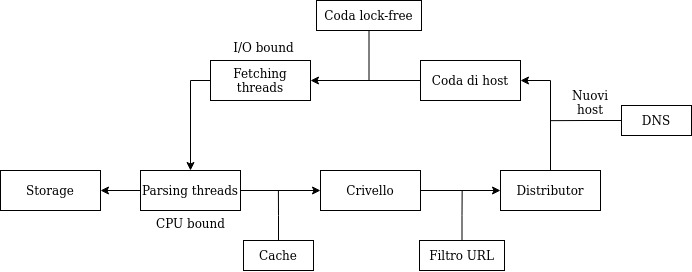
\includegraphics[width=\textwidth]{images/crawling}
    \caption{Componenti di un crawler}
\end{figure}

\subsection{Gestione parallela degli url}

\paragraph{Coordinazione agenti}
È auspicabile avere più agenti che fanno attività di crawling in parallelo, 
bisogna pensare a come distribuire il carico, un'esempio potrebbe essere quello di 
dividere per host.

Fare ciò non è molto efficiente, si può ricorrere a qualcosa di centralizzato.
Ogni agente chiede al coordinatore se tocca a lui occuparsi di un determinato host. 
Ovviamente è un single point of failure, si può pensare quindi di avere una distribuzione
del coordinatore\footnote{Un algoritmo possibile è PAXOS, una delle sue implementazioni 
è ZOOKEEPER}. Non si affronterà un algoritmo del genere, si vede ora un altro approccio.

\paragraph{Gestione statica}
Tolta la condizione di rottura degli agenti, quindi assumendo staticità, assegnare 
un url ad un agente richiede calcolare una funzione di hash modulo n, oppure 
sfruttare un approccio round robin. 

Il problema di questo approccio è che non funziona bene se gli agenti cambiano nel tempo.

\paragraph{Requisiti di gestione dinamica}

La gestione dinamica deve rispettare alcune proprietà, in particolare, si considerano
$P$ agenti, di cui $A$ agenti vivi. 

La funzione di assegnamento $\delta_A : U \rightarrow A$:
\begin{itemize}
    \item $\delta_A(u) \in A$: assegna ogni url ad un agente vivo;
    \item $\delta_A^{-1}(a) \approx \frac{|U|}{|A|}$: il carico di 
    ogni agente è circa uguale;
    \item $A \subset B \implies \delta_B^{-1}(a) \subset \delta_A^{-1}(a) \forall a \in A$: 
    aggiungendo nuovi agenti, quelli vecchi non si vedono assegnare più cose.
\end{itemize}



\paragraph{Knuth-Fisher–Yates shuffle}
Arrivato un url, creo un generatore di numeri casuali con seed pari a u. 
Permuto l'insieme $P$ di agenti e scorro finché non trovo un agente attivo $a \in A$.

Se si aggiunge un nuovo agente, gli unici url che cambiano assegnamento 
sono quelli che hanno nella lista degli agenti generata per essi, hanno un  nuovo agente che precede quello attivo selezionato precedentemente.
Quindi, gli url che cambiano posto vanno solo ad agenti nuovi.

Parto da un array lungo $n$.
Scorro l'array, all'$i$-esimo passo, seleziono una posizione $k \in [i, n-1]$ e 
scambio l'elemento $k$ e $i$.

Sono possibili $n!$ scelte, l'algoritmo genera in modo equiprobabile una permutazione possibile.

Si nota che, una volta individuato un elemento di $A$ posso fermarmi, tanto sarà
lui a gestire l'url. 
In media quindi effettuo $\frac{|A|}{|P|}$ scambi.

\paragraph{Min-hash}
Sia $u$ un url e $A$ l'insieme degli agenti, $h$ una funzione di hash. 
Un url viene assegnato all'agente $a = \argmin_{a\in A}\;h(u,a)$.

Una collisione si risolve in maniera deterministica. Questo e l'approccio
precedente sono molto simili.

\paragraph{Hashing coerente}
Un'interpretazione geometrica  è  la seguente: 
si considera una circonferenza, per ogni agente si inseriscono $C$ punti casuali 
sulla circonferenza. 
Ogni agente inizializza un seed con l'identificativo degli altri, 
generando casualmente i loro punti, quindi ogni agente ha la stessa circonferenza 
con $C$ punti per ogni $a \in A$.

Per capire dove va un url $u$, si parte dal punto definito da $h(u)$, si procede in senso orario finché non si incontra un agente.
Le repliche servono a rendere più bilanciati gli assegnamenti.

\begin{remark}
    È possibile in generale capire chi si occupava dell'url prima dell'arrivo di un 
    nuovo agente, l'approccio cambia a seconda della tecnica di hashing utilizzata, 
    nello shuffle basta procedere con l'estrazione, nel min-hashing si può mantenere 
    una finestra di k minimi. Nell'ultimo caso si può procedere nello scan della 
    circonferenza. 
\end{remark}
\newpage

\section{Retrieval}
L'attenzione passa ora alle pagine scaricate. 
Ogni documento è numerato e contiene una certa quantità di caratteri, l'obiettivo 
ora è indicizzarli.

\begin{remark}
    Tipicamente bisogna fare guessing per capire la codifica del testo, esistono 
    tabelle dedicate a questo in ogni browser.
\end{remark}

\paragraph{Segmentazione dei documenti}
Partendo da un documento di ottengono sequenze di token, in qualche modo, per esempio 
spezzando il testo agli spazi, rimuovendo le stop-words etc.
Tipicamente si applicano operazioni di normalizzazione, come troncamento, lemmatizzazione, etc.

\paragraph{Matrice termini-documenti}
Ordinando la totalità dei termini nei documenti si può ottenere una rappresentazione
matriciale con documenti sulle colonne e termini per righe. Una cella indica 
la presenza o meno di una certa parola nel testo di un documento.

Quello che si fa poi è creare la trasposta ordinata, ovvero una matrice che 
per ogni token ha una lista di interi che rappresentano i documenti in cui esso 
è contenuto.

\subsection{Codici istantanei}

Un codice è un sottoinsieme di parole binarie: $C \subseteq 2^* = \{0,1\}^*$.

\begin{definition}
    Si dice che $x$ è un prefisso di $y$, $x \preceq y$ se $\exists z \in 2^*\;t.c.\;xz = y$, ovvero se concatenato ad un altra parola binaria ottengo $y$.    
\end{definition}

\begin{definition}
    Due parole $x$ e $y$ sono confrontabili se $x \preceq y$ oppure $y \preceq x$.
\end{definition}

\begin{definition}
    Un codice $C$ si dice istantaneo se $\forall x,y \in C$, $x$ e $y$ sono inconfrontabili, ovvero privo di prefissi.
\end{definition}

\begin{definition}
    Un codice $C$ si dice completo se ogni parola binaria è confrontabile 
    con una parola $x \in C$. Ovvero, aggiungendo una qualsiasi parola binaria, 
    il codice non è più istantaneo.
\end{definition}

\paragraph{Motivazioni}
Memorizzare sequenze di interi ordinate in maniera crescente può essere fatto in maniera
efficiente memorizzando gli scarti, differenze, tra due interi consecutivi.
$$1, 6, 7, 10, 12 \longrightarrow 1, 5, 1, 3, 2$$
Queste liste potrebbero essere le righe della matrice termini-documenti.

Un'altra proprietà interessante di un codice istantaneo è l'univocità di decodifica 
scorrendo una sequenza di parole concatenate. 
Infatti, visto che nessuna parola è prefisso di un'altra, ho un solo modo di decodificare una 
sequenza di zeri e uni.

\paragraph{Ordinamento nei codici istantanei}
Due esempi di codici istantanei sono:
\begin{itemize}
    \item $k = 0^k1$
    \item $k = 1^k0$
\end{itemize}
Il secondo codice mantiene l'ordine, il secondo no.

\paragraph{Importanza della completezza}
Se un codice è istantaneo e completo si può decodificare ogni stringa binaria 
casuale in modo univoco, altrimenti no.

\subsubsection{Disuguaglianza di Kraft-Mcmillan}

\begin{definition}
    Sia $C$ un codice istantaneo, vale: 
    $$\sum_{w \in C} \frac{1}{2^{|w|}} \leq 1$$
\end{definition}
Se $C$ istantaneo, $C$ è anche completo sse $\sum_{w \in C} \frac{1}{2^{|w|}} = 1$.
Nell'interpretazione geometrica\footnote{Vedi dimostrazione} non sarebbe
libero nessun intervallo. 

\begin{remark}
    Il fatto che la sommatoria dia un valore piccolo non dice nulla su un linguaggio 
    qualsiasi, non è vera quindi l'implicazione inversa.
\end{remark}

\paragraph{Teorema interi}
Siano $t_0 \leq t_1 \leq \dots \leq t_n$ interi, se vale:
$$\sum_{i \in N} \frac{1}{2^{t_i}} \leq 1$$
Allora esiste un codice istantaneo con $n$, dove la parola i-esima ha lunghezza $t_i$.

Questo fatto rende possibile un'eventuale correzione, infatti, se avessi un codice con quelle lunghezze 
ma non fosse istantaneo, so che potrei sistemarlo.

\paragraph{Visione probabilistica}
La quantità $\frac{1}{2^{|w|}}$ si può vedere come una probabilità, visto che nel caso 
in cui un codice sia istantaneo tutte quelle quantità si sommano ad uno.

Potrei pensare di codificare probabilità maggiori a parole più corte. 
La disuguaglianza di prima, e l'algoritmo greedy associato\footnote{Non presentato qui, ma simile a Huffman}
genera il codice ottimo per una distribuzione di probabilità del tipo $\frac{1}{2}, \frac{1}{4}, \dots, \frac{1}{2^k}$.

\subsection{Esempi di codici}

\subsubsection{Codici binari}

\paragraph{Notazione binaria ridotta}
Codice binario in cui si rimuove il primo 1. Per esempio: $$1001010 \rightarrow 001010$$

\paragraph{Codice binario minimale} 
Sia $s = \lceil \log k \rceil$, se $x < 2^s - k$, esso è codificato dall'$x$-esima parola binaria
di lunghezza $s-1$, altrimenti tramite la $(x-k + 2^s)$-esima parola binaria di lunghezza $s$.



\subsubsection{Elias}

\paragraph{Codice $\gamma$}
Ogni numero è scritto in notazione binaria ridotta, ovvero in binario senza il primo uno, preceduto dalla sua rappresentazione unaria.
\begin{center}
    \begin{tabular}{|l | r | r |}
        \hline
        Numero & Codifica $\gamma$ & Unario\\
        \hline
        1 & 1 & 1\\
        2 & 010 & 01\\
        3 & 011 & 001\\ 
        4 & 00100 & 0001\\ 
        5 & 00101 & 00001\\ 
        6 & 00110 & 000001\\ 
        \dots & \dots & \dots\\
        \hline
    \end{tabular}
\end{center}

La lunghezza di $x$ nella codifica $\gamma$ è $2\lambda(x) + 1$, dove $\lambda$ è
$\lfloor \log_2 x\rfloor$.
In binario invece spenderei $\lambda(x)$, ma non è istantaneo. In unario invece 
spendo una quantità pari a $x$, che in casi in cui i numeri siano piccoli va bene, altrimenti no.

\paragraph{Codice $\delta$}
Molto simile al precedente, invece che usare l'unario, 
scrivo davanti alla rappresentazione binaria ridotta la lunghezza 
del codice $\gamma$ associato all'x-esimo numero.

Confrontando i codici visti fin'ora: 
\begin{center}
    \begin{tabular}{|l | l |}
        \hline
        Codifica & Lunghezza\\
        \hline
        Unario & $x+1 = O(x)$\\
        Elias $\gamma$ & $2\lambda (x+1) + 1$\\
        Elias $\delta$ & $2\lambda (\lambda (x+1) + 1) + 1 + \lambda(x+1)$\\ 
        \hline
    \end{tabular}
\end{center}

Il codice $\delta$ sui dice asintoticamente ottimo, visto che utilizza 
un numero logaritmico di bit più qualcosa di più piccolo. 
Nel lungo termine risparmia rispetto agli altri due codici.

\subsubsection{Golomb}

Si fissa un parametro $b$ che si dice modulo del codice. Preso un 
$x > 0$ si codifica in unario la quantità $\lfloor x/ b \rfloor$, 
seguito dalla binaria minimale di $x\;\textit{mod}\;b$.

Dato un codice, posso tornare al numero con $b\lfloor x/ b \rfloor + x\;\textit{mod}\;b$.

Fissato $b = 3$, il codice diventa 

\begin{center}
    \begin{tabular}{|l | r | r |}
        \hline
        Numero & Codifica Golomb \\
        \hline
        0 & 10\\
        1 & 110\\
        2 & 111\\ 
        3 & 010\\ 
        4 & 0110\\ 
        5 & 0111\\ 
        \dots & \dots\\
        \hline
    \end{tabular}
\end{center}

\begin{remark}
    Golomb con $b = 1$ la prima parte del codice equivale all'unario. Inoltre, questo codice ha problemi simili all'unario, 
    la prima parte infatti cresce asintoticamente come $x$, 
    nella pratica è minore, ma comunque occupa molto spazio. 
\end{remark}

\subsubsection{Codici a blocchi a lunghezza variabile}
Quello che si fa è memorizzare tanti blocchi per un singolo 
numero. Il primo bit di ogni byte contiene il fatto che 
il codice è terminato oppure no. Nel caso in cui non sia terminato 
bisogna leggere uno o più altri byte per completarlo. 

Un miglioramento è mettere tutti i bit \emph{di continuazione} 
nel primo byte, per capire fin da subito quanto proseguire.

Sio può pensare dal punto di vista logico ad una lista concatenata 
che contiene pezzi di un numero, la decodifica consiste nello scorrere 
la lista e concatenare i valori in ogni nodo.

\subsubsection{Distribuzione intesa}
Ogni codice crea implicitamente una distribuzione intesa, 
ovvero parole più corte hanno probabilità maggiore, quindi, si 
può studiare come varia questa probabilità in relazione alla lunghezza 
che assumono le parole nei vari codici.\footnote{Vedi appunti, distribuzioni intese.}

Conoscendo la distribuzione di probabilità dei dati si può utilizzare 

\subsubsection{PFOR-DELTA}
Compressione che funziona molto bene quando numeri piccoli compaiono 
molto più frequentemente di quelli grandi.

Si fissa una dimensione di blocco $B \approx 256$, la compressione avviene 
per blocchi di $B$ elementi alla volta.
Quello che si fa è scorrere gli elementi di un blocco e scegliere 
un numero di bit $b$ che rappresenti almeno una percentuale $\alpha \approx 90\%$ della totalità dei numeri del blocco. 

\paragraph{Compressione}
A questo punto scorro la lista, 
se un numero è rappresentabile in $b$ bit lo scrivo, altrimenti 
scrivo un codice di escape, per esempio tutti uni o zeri.\footnote{Necessito quindi di un valore libero per questo codice nei $b$ bit.} Accodo alla fine i numeri non rappresentabili, tutti a lunghezza $a$,
la minima per rappresentarli tutti.
All'inizio della lista inserisco il numero $b$ e il valore $a$.

\paragraph{Decompressione}
La decompressione della lista è lineare, bastano due puntatori, uno all'inizio e uno che parte 
prima dei numeri accodati.
Si ottiene una buona compressione, $b$ viene molto piccolo se tanti valori sono piccoli, inoltre nell'$alpha$-percento dei casi 
non devo accedere alla memoria accodata alla lista, che è la parte più 
costosa della decompressione.

\subsubsection{Asymmetric Numeral System}
Sono sistemi in cui cifre diverse sono scritte con numero diverso di bit, 
il che permette di scrivere numeri dove alcune cifre costano tanto, 
altre di meno.

\paragraph{Premessa}
Vorremmo che, dato un messaggio $x$, l'aggiunta di un simbolo 
che compare con probabilità $p$, crei un messaggio $x^\prime \approx \frac{x}{p}$.\\
Quindi, $\log(x^\prime) \approx \log(x) + \log(\frac{1}{p})$.
Ovvero, vorrei che, aggiungendo ad un messaggio un simbolo che compare 
frequentemente, tale messaggio si allunghi di molto poco.

La codifica binaria risponde alla richiesta precedente, dove i simboli 
sono equiprobabili.
Dato un messaggio infatti, l'aggiunta di un simbolo corrisponde a raddoppiare il valore precedente e aggiungerne uno, ovvero 
aumentare di un fattore $x/\frac{1}{2}$.

Codificando ad esempio il numero $0100110$ in decimale, quello che sto facendo sono operazioni del tipo 
$x^\prime = 2x + p$, dove $p$ è 0 oppure 1. Ciò è coerente con la premessa, 
sto aggiungendo simboli che sono equiprobabili.

\paragraph{Caso asimmetrico}
Il caso binario è semplice, codifica e decodifica si fanno 
mettendo e spostando caratteri, bisogna ora capire come fare una cosa 
simile quando la probabilità dei simboli cambia.

Siano $0,1, \dots, n-1$ simboli con una relativa probabilità associata  $p_i$.

Rappresento in maniera discreta le probabilità, considerando $2^d$ blocchi, divisi in segmenti in base alle probabilità. 
Vorrei che per ogni segmento, che ha lunghezza $f_i$, valga $f_i/2^d \approx p_i$.

Calcolo l'inizio di ogni segmento in maniera cumulativa e lo chiamo $c_i$, semplicemente sommo gli $f_j, j \leq i$.

Ogni simbolo quindi ha associato un segmento di dimensione $f_i$, lungo 
in maniera proporzionale alla sua probabilità associata.

\paragraph{Esempio}
Considero tre simboli con probabilità: $$\frac{9}{10}, \frac{1}{30}, \frac{2}{30}$$
Fisso $d$ a 10, ottengo tre blocchi lunghi $f_i$ rispettivamente: 
$$\frac{922}{1024}, \frac{34}{1024}, \frac{68}{1024}$$
Calcolo ora i $c_i$, ottengo rispettivamente: 
$$0, 922, 956$$
\begin{remark}
    Se estraggo a caso da 1024, usando i $c_i$ per capire in che segmento sono finito, 
    ottengo ogni valore quasi con le probabilità iniziali. 
\end{remark}

\paragraph{Primitive}
Definiamo ora le primitive \emph{push}, \emph{sym} e \emph{pop}:
$$\mathit{push}(x, s) = \big( \big\lfloor x/ f_s \big\rfloor << d \big)
+ c_s + \big( x\;\textit{mod}\;f_s \big)$$
Quindi, eseguo uno shift e metto nei bit più bassi quella quantità.

$$\mathit{sym}(x) = s\; | \; c_s \leq x \leq c_{s+1}$$
L'ultimo simbolo è quello associato agli ultimi $d$ bit. 

$$\mathit{pop}(x) = \langle \big(x >> d\big) \cdot f_s + \big( x\;\textit{mod}\;2^d \big) - c_s, s \rangle$$
La decodifica riporta la $x$ a prima dell'inserimento.

\subsection{Liste di affissioni, rango}
% \subsubsection{TODO: Liste di affissioni}
% \dots
\subsubsection{Riassunto processo di crawling}
Possiamo riassumere il processo di crawling come: 
\begin{enumerate}
    \item \emph{Crawling}: raccolta di pagine dal web e salvataggio
    \item \emph{Parsing}: processing dei testi, come tokenizzazione, 
    normalizzazione etc.. Ogni documento diventa quindi una sequenza di 
    token numerati. In 
    pratica si ottiene un flusso di unità da analizzare della forma 
    $$\langle\mathit{token}, \mathit{doc}, \mathit{posizione}\rangle$$
    Il tutto viene memorizzato in maniera intelligente, tramite codici 
    istantanei per ridurre lo spazio in memoria.
    Quando la memoria si riempie, scarico tutti i documenti indicizzati 
    su disco. Ottengo quindi indici inversi funzionanti per una certa 
    sequenza di documenti.
    Inoltre su disco memorizzo: 
    \begin{itemize}
        \item Liste dei termini ordinata lessicograficamente;
        \item Liste di affissioni;
        \item Lista di puntatori alle liste di affissione.
    \end{itemize}
    Successivamente fondo gli indici, che sono ordinati, con una fusione
    multivia, per ottenere l'indice totale.
\end{enumerate}

\subsubsection{Rango lessicografico efficiente}

Sono necessarie strutture efficaci per il rango lessicografico, ovvero 
per sapere l'ordine delle parole.

Si fa leva sulle strutture statiche, ovvero strutture che una volta costruite
non si cambiano. 
L'obiettivo è avere per ogni termine associato il rango, per esempio: 
\begin{equation}
    a \longrightarrow 0,
    b \longrightarrow 1,
    c \longrightarrow 2,
    d \longrightarrow 3
\end{equation}

Consideriamo ora $U$ l'insieme delle stringhe, $X \subseteq U$, i termini,
ed $f : X \longrightarrow 2^b$ la funzione che associa ad un termine il 
suo rango.
Un dizionario classico, risponde un valore se la chiave è contenuta, 
altrimenti un valore di default. Il che significa che mantiene in qualche modo 
tutte le chiavi possibili. Il che significa che un dizionario 
classico occupa almeno $$\log\bigg( \frac{|U|}{|X|} \bigg) + |X|b = \log(2^b)^{|X|}$$
Il primo termine per le chiavi, il secondo per il valore delle chiavi.

A noi interessa solo rispondere a chiavi in $X$, potremmo pensare quindi a come risparmiare spazio, occupandone solo $|X|b$, mantenendo accesso costante.

\paragraph{Idea}
Creo un sistema lineare aleatorio, lo risolviamo. 
Consideriamo $m = c|X|$ numero di variabili del sistema, dove $c > 1$. Siano ora $g, h: U \longrightarrow m$ funzioni di hash.

Per ogni chiave $x$, aggiungiamo al sistema l'equazione: 
$$V_{g(x)} \oplus  V_{h(x)} = f(x)$$

Supponiamo ora di avere una soluzione del sistema, ovvero un vettore lungo $|X|$, 
che occupa $b$ bit per ogni variabile, posso computare $f(x)$ per qualsiasi $x$, 
computando $V_{g(x)} \oplus  V_{h(x)}$.
Occupo quindi uno spazio pari a $mb = c|X|b$ più lo spazio per mantenere le funzioni 
di hash, che sono definite da qualche parametro, irrisorio rispetto al resto.

\paragraph{Risoluzione del sistema}

Costruisco un grafo dove sui nodi ho le variabili e sugli archi la variabile 
associata all'equazione.

Iterativamente efoliamo il grafo, ovvero, trovo una foglia (nodo con grado 1), sia essa 
per esempio $V_2$, collegata al nodo $V_3$.
Trovo che $V_2 = f(x) \oplus V_3$.
Stacco $V_2$, trovo un'altra foglia, proseguo così. Metto da parte quindi tante equazioni 
di quel tipo.

Prima o poi svuoto il grafo, parto dall'ultima equazione e risolvo all'indietro. 

\begin{remark}
    Questo funziona solo se il grafo è aciclico.
\end{remark}

\begin{theorem}
    Sia $m$ il numero di nodi di un grafo, $n$ il numero di archi, se vale $m \geq 2.09 n$ la probabilità che un grafo aleatorio sia aciclico tende a 1.
\end{theorem}

Il teorema precedente vale anche con un numero di nodi non troppo alto. 
Ho ottenuto quindi un modo di ottenere un grafo aciclico per far andare l'algoritmo risolutivo, 
basta usare una costante $c \geq 2.09$, fissare due funzioni e ottenere un grafo 
del sistema. Se esso presenta cicli, cambio le funzioni di hash.

\paragraph{Complicazioni}
Esistono versioni con più funzioni di hash. Se ne usassi $3$, otterrei un multigrafo, 
dove gli archi coinvolgono 3 vertici. Per quel caso la costante $c$ equivale a $1.23$.

\paragraph{Ammettere cicli}
Se si ammettono cicli bisogna ricorrere alla riduzione Gaussiana del sistema, cubica nel numero di variabili. 
Per pensare di applicarla bisogna partizionare le chiavi e risolvere sottosistemi.

\paragraph{Dire se una chiave fa parte o no di X}
Siano $S:U \longrightarrow 2^b$, $S^\prime : X \longrightarrow 2^b$. 
Creo la funzione $\bar{S^\prime}$ con la tecnica del sistema, occupando $\approx 1.23|X|b$.

Se vale $S(x) = \bar{S^\prime}(x)$ allora $x \in X$, a meno di collisioni.

\subsection{Risoluzione di interrogazioni}

L'attenzione ora passa alla risoluzione di interrogazioni a un insieme di
documenti indicizzato.

Siano ora $Q$ le query, $D$ l'insieme di documenti, vogliamo computare la seguente 
funzione: 
$$Q \times D \longrightarrow \mathbb{R}$$
che associa ad ogni documento, data una query, un punteggio.

Tra le tipologie di query posso avere ricerche ad un singolo termine, 
dove il risultato è la semantica di esso, ovvero, l'insieme dei documenti in cui il termine compare, oppure posso avere cose come unione, intersezione e negazione 
di query.

\paragraph{Query di unione}
Date più query, il risultato singolo sono insiemi di documenti, uso una fusione 
multivia\footnote{Simile al merge, ma uso un min-heap per ottenere il minimo di k liste in tempo logaritmico.} per unire i risultati.
È molto facile durante la fusione tenere traccia di quali interrogazioni hanno 
dato come risultato un certo documento, utile per effettuare ranking.

Abbiamo quindi un insieme di liste di affissione per ogni query, 
uso un'approccio pigro, ovvero, leggo il documento attuale da ogni lista, 
poi leggo l'elemento next del minimo, etc.
Questo approccio è pigro se le liste sono implementate come puntatori al prossimo.\\
Non si può fare meglio di così, ovvero, serve un numero lineare di accessi 
al next, visto che l'output contiene l'unione di tutte le liste.

\paragraph{Query di intersezione}
Consideriamo ora due query di intersezione, l'intersezione delle liste si può 
fare in tempo lineare, ma si può fare di meglio. Per esempio, 
se una fosse molto più piccola dell'altra, potrei effettuare ricerca binaria 
degli elementi della piccola nella grande.

Un'altro approccio usa ricerca esponenziale, procedo ad intervalli sempre più grandi,
appena scavalco torno all'intervallo precedente e ricomincio.
Questo approccio è vantaggioso, perché si assume che l'elemento successivo sia 
abbastanza vicino a quello corrente, cosa che capita se gli elementi della corta 
sono ben disposti in quella lunga.

Nel nostro caso non si usano questi approcci, consideriamo ora la lista corta 
che inizia con 5, quella lunga con 0, è facile capire che gli elementi della lunga
fino a quando non si incontra un 5 sono irrilevanti. Pensiamo ora alla possibilità 
di utilizzare un iteratore che non solo ha un'operazione di next, ma una di 
skip-to, che salta al maggiorante di un certo valore, in questo caso si può 
andare in tempo sub-lineare.

Nel caso in cui si abbiano $k$ liste da intersecare, si utilizza un min-heap 
per decidere la lista su cui effettuare lo skip-to, infatti, conviene far avanzare la lista più indietro, fino al massimo valore corrente. 
Se il minimo e massimo coincidono significa che esiste un intersezione.

Purtroppo nella pratica funziona meglio questo approccio: 
cerco un allineamento tra le prime due, se lo trovo allineo la terza, se non lo trovo, riallineo le prime due etc.
Quando trovo un allineamento tra le prime tre, cerco nella quarta e così via.
Il tutto funziona perché, se si ordinano gli elementi per frequenza, trovare un 
match per termini poco frequenti, ovvero match per le prime liste, farà avanzare 
le ultime di moltissimo.

\paragraph{Query di not}
Scorro la lista dei documenti, ogni volta che si incontra un buco tra gli 
elementi si emettono tutti quelli in mezzo.

\paragraph{Implementazione dello skip-to}
Mantengo in memoria un campione ogni tot elementi della lista, da decidere. 
Quando richiedo uno skip-to, ricerco in dicotomica i puntatori, poi procedo 
linearmente da quello che trovo.

\paragraph{Albero di operazioni}
Nella pratica si possono combinare unioni intersezioni e negazioni in maniera molto 
complessa, quello che si fa è, mentre si chiama next della query composta, 
tutte le sotto-query avanzano in maniera indipendente per dare in output il 
risultato complessivo.

\paragraph{Early termination}
In realtà non si completerà mai del tutto un'interrogazione, ma tramite la struttura
pigra si estraggono quanti risultati di cui ho bisogno.

\paragraph{Operatore frasale}
La query è una frase, si cercano i documenti che presentano i termini nell'ordine specificato nell'interrogazione.
L'operazione soggiacente è l'intersezione, cerco quindi documenti che hanno 
almeno tutti i termini della frase, però devo considerare anche 
la posizione dei token.
L'idea su cui si basa l'algoritmo è raccogliere le posizioni dei termini 
in un documento. 
Si ottengono quindi $k$ liste, se sottraggo alle posizioni delle liste 0, 1, 2, etc. devo risolvere una semplice intersezione. 

Si osserva comunque che l'operatore frasale potrebbe fare molto lavoro
per nulla, poichè tipicamente query frasali hanno meno risultati.

\paragraph{Operatore finestra}
La richiesta ora è trovare termini all'interno di una finestra lunga $k$, 
in qualsiasi ordine.
Si utilizza un min-heap per tenere conto della posizione dei termini 
in un documento. 

% \subsection{TODO: Punteggi endogeni}
% \dots


\section{Ranking}

% \subsection{Ranking endogeni}

\subsection{Ranking basati su distanze}

L'idea di base è quella di avere un grafo orientato di qualche tipo e associare 
un valore di importanza ai vertici osservando la sola struttura della rete.
Ogni arco è considerato un \emph{endorsement} dalla sorgente per la 
destinazione.

\paragraph{Tecnica banale}
Una delle tecniche base per misurare l'importanza di un vertice in un grafo 
è contare l'in-degree del nodo. Questa tecnica è altamente influenzabile nel 
mondo attuale, basti pensare a comprare follower, voti etc.

\subsubsection{Closeness centrality}
L'idea è considerare la somma dei cammini verso gli altri, e considerarla 
come misura di perifericità $p$. Chiaramente un nodo alla periferia di un grafo 
ha tantissime distanze grandi. La centralià $c$ è l'inverso della perifericità.
$$p(x) = \sum_{y \in N} d(x, y),\;\;c(x) = \frac{1}{\sum_{y \in N} d(x, y)}$$

Esiste anche la nozione negativa, che è diversa su un grafo orientato, più
interessante perché meno influenzabile:
$$c(x) = \frac{1}{\sum_{y \in N} d(y, x)}$$

\subsubsection{Harmonic centrality}
È necessario gestire le distanze infinite, ovvero le coppie per cui non 
esiste un cammino. Una pezza potrebbe essere considerare le sole distanze finite
nella sommatoria, però idealmente non è corretto, inoltre potrei avere casi in 
cui la centralità diminuisce all'aumentare di collegamenti entranti, che non ha 
senso.

Quello che si fa è considerare la media armonica, ovvero il totale fratto la 
somma dei reciproci delle misurazioni.
$$c(x) = \frac{1}{\frac{N}{\sum_{y \in N} \frac{1}{d(y, x)}}} \rightarrow \sum_{y \in N, x \neq y} \frac{1}{d(y, x)}$$
L'idea della formula è considerare con peso uno i vicini immediati, con peso 
$\frac{1}{2}$ quelli con distanza 2, etc.
Esistono varianti che considerano al posto dell'1 al numeratore un valore di 
peso per ogni vertice, oppure una qualche informazione esterna, per esempio 
la correlazione di un nodo verso un'altro.

\subsubsection{Betweenness}
L'idea è quella che un nodo è importante se sta in mezzo a molti cammini minimi.
Siano ora $\sigma_{yz}$ il numero di cammini minimi da $y$ a $z$ e $\sigma_{yz}(x)$ 
il numero di cammini minimi da $y$ a $z$ che passano per $x$.

La betweenness di $x$ si calcola sommando i rapporti: 
$$b(x) = \sum_{y, z \in N, y } \frac{\sigma_{yz}(x)}{\sigma_{yz}}$$

Questa misura funziona molto male in alcuni casi, per esempio in un grafo con un nodo 
che fa da bridge tra due componenti, ovvero che ha un arco verso l'una e uno verso 
l'altra, la betweenness di quel nodo sarebbe enorme, ma basterebbe un singolo arco 
tra le due componenti ad azzerarla. 
Una variante per risolvere un caso del genere è quella di considerare passeggiate 
aleatorie tra due nodi piuttosto che cammini minimi.

\subsection{Ranking spettrali}

Si parte dalla matrice di incidenza del grafo e un vettore di pesi per ogni vertice. 
Se si moltiplica il vettore per la matrice ottengo un vettore in cui il valore 
di un nodo corrisponde alla somma del peso dei predecessori.

Posso pensare di iterare il processo all'infinito, la tecnica stimerà l'autovettore 
dominante della matrice.

\paragraph{Cammini lunghi k con moltiplicazione}
Se ho una matrice dove sulle righe ho gli archi uscenti e sulle colonne quelli entranti, 
se moltiplico la matrice per se stessa ottengo in una componente $x$ $y$
il numero di cammini di lunghezza 2 da $x$ a $y$. 

Questo perché, se sulla riga $x$ ho un'uno in posizione $k$, significa che posso raggiungere 
$k$ da $x$. Nella colonna $y$ invece, un'uno in posizione $k$ implica che $k$ raggiunge $y$.
Sommare il prodotto delle componenti significa calcolare il numero di cammini del tipo 
$x \rightarrow k \rightarrow y$.

Se quindi elevo la matrice alla $k$, ottengo il numero di cammini lunghi $k$ per ogni 
coppia di nodi.

\paragraph{Numero di cammini entranti}
Se moltiplico il vettore unario per la matrice $A^k$ ottengo il numero di cammini 
lunghi $k$ entranti in ogni nodo, se inverto la moltiplicazione ottengo quelli 
uscenti.

\paragraph{Esempio}
Siano gli indici della matrice $A$ giocatori di scacchi, se $i$ ha battuto $j$ 
si troverà un 1 in posizione $A[i][j]$ e uno zero in posizione $A[j][i]$, $\frac{1}
{2}$ in entrambi
in caso di patta.

Per capire chi ha vinto basta moltiplicare la matrice per il vettore unario trasposto, 
per avere un concetto di importanza, basta eseguire moltiplicazioni del tipo 
$$A(A(\dots A\cdot 1^T))$$
L'ordine però cambia sempre, dobbiamo quindi trovare un vettore p per cui vale 
$$\lambda p = T p$$
dove $T$ è la matrice del torneo. Semplicemente $p$ è un autovettore della matrice $T$, 
con autovettore $\lambda$.

\subsubsection{Eigenvector centrality}
Considerando l'autovettore dominante di una matrice che rappresenta un grafo, 
possiamo considerare la componente di valore massimo come il nodo più centrale del grafo.
La computazione di basa sul \emph{power method}, e il senso è quello di considerare come punteggio di un nodo la somma dei punteggi di chi lo punta, e continuare a 
raffinare questo punteggio continuando a ricalcolare.

\begin{theorem}
    Sia $A$ una matrice con tutte le componenti non negative e il grafo definito da $A$
    fortemente connesso, $\forall i,j\;\exists\;k\;t.c\; (A)^k_{ij} > 0$. 
    Per una matrice di questo tipo esiste un solo autovalore dominante reale positivo, 
    con autovettore associato maggiore di zero.
\end{theorem}

\subsubsection{Catena di Markov}
Si considera un grafo orientato pesato. I pesi sugli archi rappresentano la probabilità 
di transizione da una sorgente a una destinazione, la somma dei pesi degli archi 
uscenti da ogni nodo è uno.
Possiamo al solito rappresentare il grafo con una matrice, dove la somma di ogni riga 
è uno.

Per calcolare la probabilità di esser in un nodo si sommando le probabilità di 
essere in uno dei predecessori, moltiplicata per il peso dell'arco verso il nodo stesso.
Il processo appena descritto corrisponde al moltiplicare la probabilità attuale 
per la matrice del grafo.

La distribuzione stabile si calcola quindi iterando la moltiplicazione della matrice 
per una distribuzione iniziale. La distribuzione stabile contiene
la probabilità, interrompendo una camminata casuale sul grafo, di trovarsi un determinato 
nodo. 

Esistono casi strani, per esempio due nodi connessi tra loro, in tal caso 
la massa di probabilità fa ping-pong tra i due nodi, non portando a un risultato 
utile.

\subsubsection{PageRank}
L'idea è quella di avere un random surfer nel web, ad ogni passo si tira una 
moneta di peso $\alpha$ e se esce testa si visita una pagina casuale, 
altrimenti si procede nel grafo del web.
Si procede quindi come una catena di Markov classica ma ogni tanto si salta.
In realtà, si può anche fare qualcosa di più fine riguardo al saltare casualmente, 
ovvero, potrei muovermi verso siti che trattano lo stesso argomento di quello
attuale.

Al solito, quello che si vuole trovare è il vettore stabile di questa catena, 
che è l'autovettore dominante.
L'introduzione del salto casuale corrisponde di fatto ad aggiungere tutti gli archi 
mancanti al grafo, rendendolo una cricca.

\subsection{Metodi computazionali}

\paragraph{Calcolo autovettore}
Per calcolare un autovettore si parte da un array iniziale $r_0$, quello unitario per esempio, 
oppure nel caso di PageRank tutto a $\frac{1}{n}$. moltiplico per la matrice $M$, fino 
a che due risultati consecutivi differiscono, in qualche norma, di una quantità minore 
di $\epsilon$, ovvero $||r_{i} - r_{i-1}|| < \epsilon$.

La matrice $M$ non è in memoria ma memorizzata in memoria in qualche modo, per esempio
triplette $(i,j, M[i][j])$ ordinate.

Assumendo che la matrice arrivi colonna per colonna, quello che si fa è moltiplicare 
il vettore $r_i$ attuale per la colonna, volendo in multiprocessing, assumendo che la 
variabile che mantiene il risultato sia incrementabile atomicamente. 
È necessario però avere il grado dei predecessori, per esempio per PageRank, 
si deve mantenere quindi il grado per ogni riga in memoria.

Se la matrice arrivasse per riga, dovrei calcolare il prodotto riga colonna a pezzi, 
mantenendo i risultati parziali in un vettore.




\end{document}